\documentclass{sn-jnl}                  % Between authors
%\documentclass[referee]{sn-jnl}        % For referees

% Meta Info
\jyear{2023}

% Allow bottom of page to be ragged
\raggedbottom

% Use APA style
\usepackage[natbibapa]{apacite}
\AtBeginDocument{
    % Turn off "Retrieved from " for URL
    \renewcommand{\BRetrievedFrom}{$\!\!$}
    % Turn off "doi: " for DOI
    \renewcommand{\doiprefix}{$\!\!$}
    % Format DOI as "https://doi.org/10.xxxx/xxxx" clickable
    \renewcommand{\doi}[1]{\href{https://doi.org/#1}{https://doi.org/#1}}
}

\usepackage[nameinlink,capitalise]{cleveref}
% Must be the last package loaded

\begin{document}

\title[Family Factors and Adolescent Antisocial Behavior]{Parental Mental Distress and Adolescent Antisocial Behavior: The Mediating Role of Family Conflict and Cohesion}

\author[1]{\fnm{Frida T.} \sur{Skancke}}\email{frida.skancke@isp.uio.no}
\author[1]{\fnm{Thea Fahle} \sur{Mausethagen}}\email{thea.mausethagen@isp.uio.no}
\author[2]{\fnm{Tony C. A.} \sur{Tan}}\email{tctan@uio.no}
\equalcont{These authors contributed equally to this work.}
\author[3]{\fnm{Agathe} \sur{Backer-Gr{\o}ndahl}}\email{agathe.backer-grondahl@nubu.no}
\author*[{1,3}]{\fnm{Gunnar} \sur{Bj{\o}rnebekk}}\email{gunnar.bjornebekk@isp.uio.no}

\affil*[1]{\orgdiv{Department of Special Education}, \orgname{University of Oslo}, \orgaddress{\street{PO Box 1140}, \city{Blindern}, \postcode{0318}, \state{Oslo}, \country{Norway}}}
\affil[2]{\orgdiv{Centre for Educational Measurement}, \orgname{University of Oslo}, \orgaddress{\street{PO Box 1161}, \city{Forskningsparken}, \postcode{0318}, \state{Oslo}, \country{Norway}}}
\affil[3]{\orgdiv{Forskningsavdelingen}, \orgname{Norwegian Center for Child Behavioral Development}, \orgaddress{\street{PO Box 7053}, \city{Majorstuen}, \postcode{0306}, \state{Oslo}, \country{Norway}}}

\abstract{Antisocial behavior (ASB) has profound consequences for both the individuals and the society. Research efforts therefore keenly focus on the latent mechanisms contributing to individuals' ASB tendency. Although the direct relationship between parents' mental distress and adolescents' ASB is well documented, we further interrogate whether such assosications can be partially explained through family conflict and cohesion as mediating factors. We studied 157 adolescents and their primary caregivers using a Norwegian clinical sample, with mean ages of 14.74 (range 11--18) and 43.93 (range 29--78) for the diad respectively. Our structural equation models revealed a significant mediating effect between parental mental distress and adolescent ASB through family conflict. This result suggests a covariation among high parental symptoms of depression and anxiety, hightened conflict within the family, and increased aggressive and rule-breaking behavior among the adolescents under their care. Having controlled for the family conflict pathway, we no longer find significant mediating effect via family cohesion. Our study contributes to literature by not only reaffirming the significant roles parental mental distress and family conditions play on adolescents ASB, but also by demonstrating the structural mechanism among these factors.}

\keywords{adolescent antisocial behavior (ASB), parental mental distress, family conflict, family cohesion, mediation}

\maketitle

\section{Introduction}

Parental mental distress is found to be connected to maladjustment and problem behaviors in children and adolescents \citep{elgar:2007, joyner:2021}. Factors in the family environment and interpersonal relationships between family members are highlighted as certain aspects that may exacerbate this influence, and is therefore important to consider as underlying factors and triggers for adolescent outcomes \citep{vanloon:2014, xu:2017}.

\subsection{Adolescent Antisocial Behavior}

Antisocial behavior (ASB) is characterized as behaviors that violate norms and rules about how persons and property should be treated \citep{scott:2015}. These behaviors are destructive and insensitive to other people's rights, it can be criminal and noncriminal, overt and covert, and may include aggression, substance use, bullying, sexual precocity, and vandalism \citep{dishion:2006}. Criminal behavior in childhood and adolescence is referred to as delinquency \citep{hiatt:2008}. Clinical diagnoses, like oppositional defiant disorder (ODD), and conduct disorder (CD) are used to describe antisocial behavior in literature \citep{fonagy:2021}.

Persistent ASB can have major long-term consequences both for the individual and society \citep{lobraico:2020}, such as academic failure, drug abuse, violence, and economic struggle \citep{moffitt:2001, moffitt:2018}. Exhibition of ASB is heterogeneous, but one of the most common forms of behavioral problems during childhood and adolescence \citep{frick:2009}. Early emerging ASB in childhood have a higher chance of persisting into adulthood, due to more severe individual and environmental risk factors. Maternal psychopathology, harsh and neglectful parenting, and elevated family conflict are some of such factors \citep{dishion:2006, moffitt:2015}. However, for youth who participates in ASB in adolescence tend to have more normative backgrounds (e.g., socioeconomic status and family risk), compared to the early starters \citep{moffitt:2001}.

Growing research advocates for distinguishing between different subtypes for adolescent ASB \citep{burt:2012, burt:2009, kornienko:2019}. The main distinction is between aggressive (e.g., verbal, physical aggression, bullying and violence) and non-aggressive behaviors (e.g., theft, vandalism, and relational aggression) \citep{burt:2016, kornienko:2019, little:2003}. Some also include risk-taking behaviors \citep{mishra:2008}, defined as engagement in actions that are associated with potentially adverse consequences \citep{boyer:2006}. Risk-taking behaviors are thought of as more normative in adolescence \citep{moffitt:2018, sundell:2019}, they are not necessarily illegal or dangerous, but include actions where the outcome is uncertain \citep{ciranka:2021}. Lastly, \citet{steinberg:2004} points out that adolescents are  susceptible to peer pressure, making them more likely to engage in similar activities and behaviors as their peers \citep{ciranka:2021}.

\subsection{Parental Mental Distress}

Several mechanisms, such as genes \citep{burt:2003, moffitt:2015}, individual temperament \citep{dadds:2003}, modeling \citep{garber:2005, vanloon:2014}, parenting practices \citep{romm:2022, sun:2021}, and family climate \citep{cummings:2000, patterson:2002} have been found to elevate risk for adolescents ASB \citep{fosco:2019}. The connection between parental mental distress, symptoms of depression and anxiety, are well established risk factors for child and adolescent outcomes \citep[e.g., ][]{cummings:1994, goodman:2006, hails:2018, hawes:2005}, indicating that mental distress may reduce parents' ability to engage in proactive and positive parenting \citep{elgar:2007, joyner:2021}. Conversely, research has found a transactional influence between parental mental distress and offspring behavioral problems, indicating that higher levels of adolescent ASB are associated with chronic trajectories of mental distress in parents \citep{elgar:2007, korhonen:2014, xu:2017}.

Family environments with depressed caregivers are characterized by negative patterns of interpersonal interactions, lax monitoring, and inconsistent discipline and display of affection \citep{elgar:2007, korhonen:2014}. Cummings and colleagues (\citeyear{cummings:2005}) found that parental depressive symptoms were linked to poor child adjustment, both internalizing and externalizing problems, peer rejection and lack of prosocial behavior, and that greater parental symptoms were associated with intrusiveness, control through guilt, and less parental warmth. Parents' mental distress increased parental rejection and overprotection, which in turn functioned as a mediator between parental psychopathology and offspring ASB \citep{vera:2012}. \citet{korhonen:2014} investigated whether it is the timing, recurrence or chronicity of maternal depression that puts offspring's wellbeing at risk. Findings indicate that recurrent depressive symptoms were significantly associated with adolescents' poorer psychosocial health, including self-reported externalizing behaviors. Anxious parents are often more controlling and overprotective, they tend to parent their offspring's closely, expecting disclosure of information, and allowing less autonomy \citep{jones:2021, vera:2012}. Anxiety symptoms in mothers are associated with negative criticism \citep{hirshfeld:1997}, and lower levels of affirmation towards their adolescent, which in turn predict higher levels of externalizing behaviors \citep{bellina:2020}.

Research is somewhat conflicted on the role of mothers and fathers separate influence on offspring adjustment, and less focus have been on the influence and role of paternal mental distress \citep{cummings:2005, sweeney:2016}. Notably, both \citet{marmorstein:2004} and Vera and colleagues (\citeyear{vera:2012}) found that mothers had a greater influence on child outcomes, with higher levels of maternal mental distress predicting higher levels of maladjustment in offspring compared to fathers. Conversely, a meta-analysis conducted by \citet{connell:2002} did not find differences in mothers' and fathers' psychopathology on externalizing behavior. However, they found that parents' gender may predict internalizing behavior, with mothers having a greater influence.

\subsection{Family Conflict and Cohesion as Mediators}

Parental mental distress may function as a risk factor for increased conflict levels and lower levels of cohesion within families. Family conflict involves frequent expression of anger, hostility, and resentment \citep{lobraico:2020}.  Adolescents' desire for autonomy and liberation from parental control in adolescence may be a source for frustration, friction, and conflict \citep{buehler:2006, saxbe:2014}. Conflict between parents and offspring tends to increase during adolescent years, peaking during early adolescence, as they attempt to adjust boundaries, renegotiate parental authority, and increase their own autonomy and independence \citep{weymouth:2016}. High levels of family conflict are associated with emotional and behavioral problems, such as symptoms of mental distress, aggression, delinquency, and school problems \citep{fosco:2020, sun:2021, xu:2017}. A meta-analysis by Weymouth and colleagues (\citeyear{weymouth:2016}) found positive associations between parent-adolescent conflict and youth maladjustment. Similar results were found by \citet{xu:2017}, with increased family conflict, as reported by both parent and youth, resulted in higher risk for adolescent maladjustment. Family conflict is also connected to risky behavior, with increased conflict leading to heightened engagement in risky behaviors \citep{skinner:2016}. Further, \citet{romm:2022} found that love withdrawal was strongly associated with greater substance use, delinquency, physical and relational aggression. Showing that parental rejection may result in anger and frustration, as well as difficulties in emotional coping. Elevated levels of conflict may increase the use of coercive strategies in parent-adolescent interactions \citep{lobraico:2020}. In families where coercive interactions dominate, ASB emerges and then stabilizes over time \citep{granic:2006}.

Family climate may function as a buffer (or protective factor) against adolescents ASB. Family cohesion is characterized by warmth, openness, emotional connection, and flexibility, and offspring in such families are found to have better psychological and behavioral adjustment than conflicted families, that are more distant, hostile, and aggressive \citep{coe:2018, richmond:2006, sun:2021}. High and stable levels of cohesion make family members less adversely affected by parental mental distress, adolescent ASB, or other life challenges \citep{coe:2018}. Adolescents who feel connected to their family, are more likely to seek guidance and disclose information to their parents, and spend time with their families, leaving them with less opportunity to affiliate with delinquent and deviant peers \citep{fosco:2019, vieno:2009}. During adolescence, family cohesion tend to decrease \citep{dekovic:2003, lin:2019}. This decrease can be interpreted by adolescent development and liberation processes \citep{baer:2002}.  \citet{lin:2019} found decreasing levels of family cohesion in Taiwanese youth. The decrease was lower and had less impact on the teenagers who initially reported high levels of cohesion, while low family cohesion in early adolescence resulted in more delinquent behavior later in adolescence. Likewise, \citet{coe:2018} and \citet{richmond:2006} found that low family cohesion was a predictor for externalizing behavior in forms of conduct problems, oppositional defiance, and hostility.

Depressed mothers report that their family environments more often are less cohesive and more conflict-filled, compared to non-affected mothers \citep{slee:1996}. P{\'e}rez and colleagues (\citeyear{perez:2018}) report that higher levels of maternal depression were associated with lower levels of family cohesion, reported by both mother and adolescent. \citet{fosco:2020} found that adolescents within families with high levels of cohesion, reported feeling more positive, more satisfied with life, and less angry, depressed, and anxious. Reflecting that family cohesion can function as a protective factor against life difficulties.

\subsection{The Current Study}

In the current study, we aim to investigate whether family conflict and cohesion mediate the effect of parental mental distress on adolescent antisocial behavior. We hypothesize that higher symptoms of parental mental distress will increase levels of family conflict and decrease levels of family cohesion. Further, we hypothesize that elevated levels of family conflict is related to increased adolescent ASB, while elevated levels of cohesion is associated with lower adolescent ASB. We also expect a covariance between the two mediators, with high levels in one resulting in low levels in the other. In addition, we expect to find an indirect effect from parental mental distress via family conflict and cohesion on adolescent ASB.

\section{Methods}

\subsection{Participants}

The current study utilized data from a randomized controlled trail of functional family therapy (FFT) in Norway \citep{bjornebekk:2013}. Adolescents and caregivers from 159 families participated in a combined randomized control- and process-outcome design which south to treat moderate to severe antisocial behavior \citep{bjornebekk:2013}. The inclusion criteria were (a) adolescents between 11 and 19 years, (b) which displayed, or were at risk for, one or several behavioral problems: aggressive (both verbal and physical) and violent behavior, (c) delinquency with severe risk for future offences, (d) vandalism, (e) severe rule breaking behavior at home, school or in the local community, and (f) substance use. Exclusion criteria were (a) adolescents with autism spectrum disorder, (b) imminent risk of suicide or had recently experienced an acute psychotic episode. Additionally, (c) home environments considered unsafe for the therapist, (d) cases with ongoing investigation by the local child welfare service, and (e) cases that already participated in interventions or treatments that were incompatible with FFT were also excluded.
Two observations were removed due to complete absence of information, leading to an eligible sample size of 157 adolescents (age $M = 14.74$, $SD = 1.47$, range = [10.80, 17.88]) and their primary caregiver (age $M = 43.93$, $SD = 6.90$, range = [29, 78]). There was a slightly higher proportion of male adolescents ($n=85$, 52.1\%) compared to females ($n=72$, 45.9\%) while proportions reversed for caregivers with 89.8\% mothers and 10.2\% fathers ($n=141$, $n=16$) respectively. Most adolescents lived with single parents ($n=59$, 37.6\%), while the remaining lived with both parents, adoptive parents, or in foster care (see \cref{tab:demographic}).

\subsection{Procedures}

Participants were measured at three points: T1---before participants were sampled into different groups, T2---after intervention/treatment, and T3---follow-up one year after intervention/treatment. The current study utilized data from the first point of measure (T1), making it a cross-sectional design. Resultantly, the relationships between the study variables will not be affected by intervention/treatment.

Both parents and adolescents completed all questionnaires on portable computers, programmed in \textsf{Ci3} software \citep{sawtooth:2013}. The participants completed the questionnaires in their homes, or at a municipality office. A research assistant was available for assistance and gave general instructions on how to use the \textsf{Ci3} system. Families received a minor compensation for participation \citep[equivalent to 50 USD][]{thogersen:2020}.

\subsection{Measures}

\subsubsection{Asolescent Antisocial Behavior (ASB)}

Child Behavior Checklist 6--18 \citep[CBCL, ][]{achenbach:2001} was used to assess adolescent ASB. This is one of the most used parental measures of emotional and behavioral problems among youth ages 6-18 years. Based on their adolescent's behavior over the past six months, primary caregivers filled out 113 CBCL items in 3-point Likert scales: 0 (not true), 1 (true or sometimes true), and 2 (very true or often true) \citep{achenbach:2001}. Historically, CBCL has shown acceptable reliability and validity \citep{achenbach:2001, naarking:2004, pandolfi:2014}, also in Norwegian samples \citep{lurie:2006}. To measure the outcome variable ASB, we used the subscale ``externalizing behavior'' that consists of two syndrome scales: ``aggressive behavior'' (``Attacks other people physically'') and ``rule-breaking behavior” (``Breaks rules at home, at school, or other places'') \citep{achenbach:2001}. Parent-reported ASB has satisfactory reliability with externalizing behavior (35 items; $\alpha = .92$), aggressive behavior (18 items; $\alpha = .92$), and rule-breaking behavior (17 items, $\alpha = .81$), respectively.

\subsubsection{Parental Mental Distress}

The Norwegian version of Symptoms Checklist (SCL-8) was used to measure parental mental distress. This is a brief, self-reported questionnaire measuring mental illness and distress \citep{fink:2004a}. SCL-8 is a short version of the \textit{Hopkins Symptom Checklist} \citep[SCL-90][]{derogatis:1974}, which is a well-designed assessment for overall mental distress \citep{siqveland:2016}. Parents answer eight items about the presence and intensity related to symptoms of anxiety and depression the last 14 days (e.g., ``Sudden fear without any clear reason''), on a 4-point Likert scale: 1 (Not bothered), 2 (Somewhat bothered), 3 (Very bothered) and 4 (Very much bothered). The SCL-8 scale contains only emotional symptoms, and is suggested to be a valid and robust, brief screening tool \citep{fink:2004a, fink:2004b} with high reliability (8 items, $\alpha = .91$).

\subsubsection{Family Conflict and Cohesion}

Family conflict and cohesion were measured using parental self-report of the Norwegian version of the Family Environment Scale (FES), which assesses the social environment of families along ten salient dimensions \citep{moos:1976}. FES consists of 90 true/false items distributed onto ten subscales, with conflict and cohesion consisting of nine items each. Conflict is conceptualized as the amount of openly expressed anger and aggression, and how conflicted interactions are characteristics of the family (``Family members often criticize each other''). The cohesion subscale is operationalized as the extent family members are concerned and committed to the family and the degree of support and helpfulness between family members (``Family members really help and support one another'') \citep{moos:1976, lucia:2006}. Results are somewhat conflicted on the acceptable validity and reliability of FES \citep{moos:1990, moos:2009, roosa:1990}. Our analysis found acceptable reliability for both the conflict and cohesion subscales ($\alpha = .76$ and $\alpha = .73$, respectively).

\subsubsection{Control Variables}

Adolescent age and gender were included as control variables. In addition, for parents, their interpretation of economic hardship, and educational level were controlled for. Economic hardship was measured on a 5-point Likert scale: 1 (living comfortably), 2 (Doing alright), 3 (Just about getting it), 4 (Finding it quite difficult), and 5 (Finding it very difficult). Parental educational level was measured on a 3-point Likert scale: 1 (Primary and secondary school), 2 (Upper secondary school), and 3 (Higher education).

\subsubsection{Ethical Considerations}

The current study received approval from the Regional Committees for Medical and Health Research Ethics (REK) to utilize data gathered by the study of Evaluation of FFT in Norway \citep{bjornebekk:2013}. Both parents and adolescents participants gave their informed written consent. Consent forms included information about participants' right to withdraw from the study at any given time without any adverse consequences, and safeguard of participants' confidentiality. Participants consent forms were presented for Norwegian Center for Research Data (NSD) and Norwegian Data Protection Authority (Datatilsynet) \citep{bjornebekk:2013}. All data were collected, stored, and processed within a certified secure IT environment \citep[TSD, ][]{tsd:2020}.

\subsubsection{Data Analysis}

A mediation analysis is suitable to examine how or if one variable is related to another variable through some other variable. We proposed a structural equation model (SEM) with two mediators \citep{mackinnon:2008, rucker:2011}. We firstly conducted series of preliminary analyses using \textsf{SPSS} 28, including descriptive statistics, missing values, and correlation studies. All variables appeared to be non-normal based on Shapiro-Wilks test: parental mental distress ($W = .92$, $p < .001$), adolescent ASB ($W = .98$, $p < .05$), family conflict ($W = .94$, $p < .001$), family cohesion ($W = .92$, $p < .001$), and economic hardship ($W = .88$, $p < .001$). Resultantly, we reported correlations in Spearman's $\rho$. Two observations were removed before analysis due to whole-row missings. Next, we carried out SEM analyses in \textsf{Mplus} \citep[Version 8.3, ][]{muthen:2017} to examine direct and indirect effects among parental mental distress, adolescent ASB, family conflict, and cohesion. In order to account for missing data, ten imputed datasets were generated using \textsf{Mplus}'s unrestricted variance-covariance model \citep[``JM-AM H1'',][]{asparouhov:2022}. The path between parental mental distress, family conflict, and adolescent ASB was controlled for by economic hardship (see \cref{tab:results}). We employed robust maximum likelihood (MLR) estimator due to its ability to handle non-normal data, as well as Bayes estimators for corroboration. Model fit was evaluated using SRMR. Standardized parameter estimates were used to assess the direct and indirect effects between variables.

\section{Results}

\subsection{Descriptive Statistics}

Means, standard deviations, and correlations between all study variables are presented in Table 2. Due to non-significant correlations with the proposed control variables, adolescent age, gender, and parental educational level, they are not reported in text. However, economic hardship correlated with both parental mental distress ($\rho = .17$, $p = .031$, $95\% \text{ CI} = [.012, .326]$), and family conflict ($\rho = .20$, $p = .013$, $95\% \text{ CI} = [.037, .352]$). We therefore included economic hardship as a relevant variable. Correlations show that parental mental distress were significantly associated with adolescent ASB ($\rho = .42$, $p < .001$, $95\% \text{ CI} = [0.27, 0.55]$). Parental mental distress was significant with family conflict ($\rho = .46$, $p < .001$, $95\% \text{ CI} = [0.32, 0.48]$), and family cohesion ($\rho = .28$, $p < .001$, $95\% \text{ CI} = [-0.43, -0.12]$). Adolescent ASB was significant with family conflict ($\rho = .38$, $p < .001$, $95\% \text{ CI} = [0.23, 0.52]$), and cohesion ($\rho = -.24$, $p < .001$, $95\% \text{ CI} = [-0.39, -0.08]$). The two mediating variables correlated strongly ($\rho = -.45$, $p < .001$, $95\% \text{ CI} = [-0.57, -0.31]$).

\subsection{Mediation Analysis}

To investigate the effect of family conflict and cohesion on the relationship between parental mental distress and adolescent ASB, a multiple mediation analysis was performed using \textsf{Mplus}. The outcome variable for the analysis was adolescent ASB, while the predictor variable was parental mental distress. The two mediating variables were family conflict and cohesion. Due to sample size constraint, manifest rather than latent variables were utilized in the model. In this analysis we explicitly allow the two mediators to covary to account for their oriented dependence. Family conflict and cohesion had a significant negative covariance ($\hat{\rho} = -.37$, $SE = 0.07$, $p < .001$, $95\% \text{ CI} = [-0.51, -0.24]$). Model fit indices suggest good fit, considering the small sample size (RMSEA = 0.00, $p$ = .863, CFI = 1.00, TLI = 1.10).

\subsection{Direct Effects}

Parental mental distress was significantly related to adolescent ASB ($\hat{\beta} = .29$, $SE = 0.08$, $p < .001$, $95\% \text{ CI} = [0.14, 0.44]$). As shown in \cref{fig:result}, the path between parental mental distress and family conflict was significant ($\hat{\beta} = .39$, $SE = 0.07$, $p < .001$, $95\% \text{ CI} = [0.24, 0.53]$), so was that from parental mental distress to family cohesion ($\hat{\beta} = -.30$, $SE = 0.07$, $p < .001$, $95\% \text{ CI} = [-0.44, -0.16]$). The path between family conflict and adolescent ASB was significant ($\hat{\beta} = .23$, $SE = 0.08$, $p < .001$, $95\% \text{ CI} = [0.13, 0.44]$), while to family cohesion was not ($\hat{\beta} = -.05$, $SE = 0.07$, $p = .459$, $95\% \text{ CI} = [-0.19, 0.09]$). We controlled for economic hardship, which was significant on parental mental distress ($\hat{\beta} = .18$, $SE = 0.09$, $p < .05$, $95\% \text{ CI} = [0.01, 0.35]$), family conflict ($\hat{\beta} = .13$, $SE = 0.06$, $p < .05$, $95\% \text{ CI} = [0.02, 0.24]$), but not on adolescent ASB ($\hat{\beta} = -.14$, $SE = 0.08$, $p = .061$, $95\% \text{ CI} = [-0.29, 0.01]$).

\subsection{Indirect Effects}

The indirect mediation of family conflict on parental mental distress and adolescent ASB was significant and positive ($\hat{\beta} = .11$, $SE = 0.04$, $p < .05$, $95\% \text{ CI} = [0.09, 0.43]$). In contrast, the indirect mediation path of family cohesion between parental mental distress and adolescent ASB failed to reach significance ($\hat{\beta} = .02$, $SE = 0.02$, $p = .461$, $95\% \text{ CI} = [-0.06, 0.14]$). The total indirect mediation, including both conflict and cohesion, showed a significant total indirect effect ($\hat{\beta} = .12$, $SE = 0.04$, $p < .001$, $95\% \text{ CI} = [0.05, 0.20]$).

\begin{figure}[t]
    \centering
    \includegraphics[width=\textwidth]{result.eps}
    \caption{Structural Equation Model Parameters}
    \label{fig:result}
    % Add figure note
    \begin{minipage}{\textwidth}
        \smallskip % Insert a small skip between caption and note
        \footnotesize % Reduce note font size
        \textit{Note.} This structural equation model predicts youth's antisocial behavior (ASB) from parental mental health (PMH), with mediating effects from family conflict (CON) and family cohesion (COH). Variables in ellipses are latent constructs (see \cref{app:latent}). Parameters are reported as standardized regression coefficients pooled over ten imputed datasets \citep{little:2020,vanbuuren:2018}, computed using Bayes estimator \citep{depaoli:2021}. Solid lines are visualized in proportion to their estimates while dashed lines represent nonsignificant relations at $\alpha=.05$ level. Socioeconomic status (SES) forms serial mediations with PMH, CON, and COH \citep[Model 81,][p. 643]{hayes:2022}. Control variables are drawn in grey and are all nonsignificant.\\
        $^* p < .05$. $^{**} p < .01$. $^{***} p < .001$.
    \end{minipage}
\end{figure}

\section{Discussion}

The current study aimed to investigate whether family conflict and cohesion have any mediating role on the relationship between parental mental distress, and adolescent ASB measured by parent-reported symptoms of depression and anxiety, and aggression and rule-breaking behavior, respectively. First, we hypothesized that there would be a direct association between parental mental distress and adolescents ASB. Second, we hypothesized that elevated levels of mental distress among parents to be correlated with increased conflict and lower cohesion. Third, we expected elevated levels of conflict to be associated with heightened adolescent ASB, while cohesion would have the opposite effect. Mediation analysis revealed that parental mental distress had a direct effect on adolescent ASB. Further, we found that family conflict had a mediating role in the relation between parental mental distress and adolescent ASB, while cohesion was not a significant mediator.

Analysis supported our first hypothesis and is consistent with previous research. This suggests that parental mental impairments are related to adolescents ASB, and that this relationship is only partially mediated \citep{vera:2012, kane:2004, korhonen:2014}. Indicating that parental mental distress, with all the possible behaviors or attitudes this measure includes, have a direct effect on offspring's ASB. However, we can not exclude other alternative mechanisms as possible causes and links between parental mental distress and adolescent ASB. Possible mechanisms may include parenting styles and behaviors \citep{hautmann:2015, vera:2012}, parental hostility and overprotection \citep{sellers:2014}, and coping strategies \citep{francisco:2015}. Environmental factors outside the family, such as peer relationships, and neighborhood, may also influence the relationship between parental mental distress and adolescent outcomes. In regards to a reciprocal perspective, \citet{gross:2009} found that noncompliance in offspring was the most robust predictor for higher and more persistent levels of depressive symptoms among mothers, showing that living with aggressive and rule-breaking adolescents may elevate parental distress.

As to the second hypothesis, we found that elevated levels of parental mental distress is associated with increased levels of family conflict, and a reduction in family cohesion. These results were also consistent with previous findings \citep{garber:2005, perez:2018, xu:2017}. We assume that the parents' mental impairment negatively affects their ability to choose proactive and effective parenting strategies. As previous research has found that depressed caregivers use inconsistent discipline, initiate negative patterns of interactions, and lack of monitoring \citep{korhonen:2014}. Further, this may explain why family environments with distressed caregivers may function as catalysts for adverse interaction patterns, resulting in chronic conflict-filled communication between family members \citep{garber:2005}. \citet{lobraico:2020} identified subgroups of family constellations of family risk for long-term adolescent ASB, with results indicating that adolescents in coercive families experienced the most robust risk across ASB outcomes. These families were characterized by high family conflict and low positive family climate, parental involvement, effective discipline, parental knowledge, and adolescent positive engagement.

Unsurprisingly, when there are elevated and chronic patterns of conflict among family members, and within specific dyads, such as between parent and adolescent, family cohesion deteriorates. Interpersonal relationships characterized by hostility and conflict can result in withdrawal by family members \citep{romm:2022}. In line with previous research \citep{li:2021, vanloon:2014}, we also found that higher levels of depression and anxiety in parents were associated with lower levels of family cohesion. In general, family cohesion levels tend to decrease during adolescence as they seek liberation and autonomy \citep{baer:2002, lin:2019}. However, it is reasonable to assume that within a clinical sample, with interactions characterized by high conflict and mental impairment among parents, any deterioration in family cohesion will escalate the situation. This view is in agreement with the transactional perspective on psychopathology, where high levels of family conflict and low family cohesion may exacerbate parental mental distress.

Regarding our third hypothesis, overall results indicate that family conflict has a mediating role on the relationship between parental mental distress and adolescent ASB, while cohesion does not. There are several explanations for why and how family conflict has an impact on the path to adolescent ASB. Parents with increased mental distress usually have reduced capacity and ability to engage in positive and favorable parenting \citep{joyner:2021}. As depression and anxiety influence parenting styles characterized by control through guilt and overprotection, hostility, criticism, and inconsistent discipline \citep{cummings:2005, korhonen:2014}. This may result in a family environment characterized by coercive and hostile attitudes and behaviors. Families that engage in more hostile behaviors, in the form of fighting and aggression, may damage both trust and secure attachments between parent and adolescent \citep{buehler:2006, weymouth:2016}. When this pattern of communication becomes normative between family members, offsprings may adopt this pattern of interacting on her or his social arenas. Thus, aggressive and antisocial patterns of interaction become stable in all social relations, encouraging affiliation with antisocial groups and peers \citep{carroll:2009, moffitt:2015}.

Adolescence brings normative shifts in family relations, resulting in increased conflict between parent and youth, as most youth attempt to adjust boundaries, renegotiate parental authority, and increase their own autonomy and independence \citep{weymouth:2016}. Additionally, during adolescence, youth tend to be more oppositional \citep{steinberg:2011}, which may further exacerbate adverse patterns of communication and interaction. Developmental trends like these become more problematic for mental distressed parents, compared to non-distressed. A possible explanation may be that conflicted interests between parent and adolescent, with adolescents being autonomy seeking and parents autonomy limiting, results in more friction and conflict within the family environment and their relationship. As such, family conflict can become the environmental manifestation of parental mental distress, which contributes and escalates  adolescent ASB.

As we expected, the two mediating factors negatively covary. This implies that high reading in one mediator is associated with decrease in the other one. In our sample this is noticeable on parental reports of high family conflict reducing the appearance of cohesion. We assume that due to a clinical sample referred to family therapy, that the levels of conflict reflect a more turbulent family situation compared to the general population, with frequent and coercive patterns of interaction. In addition, it is possible that adolescents' problem behavior and engagement in antisocial activities results in more friction and unfortunate communication with their parents. Also, mental distress among parents is associated with reduced levels of family cohesion \citep{perez:2018}, with mental distress influencing parents' ability to positively and affectionately engage with their offspring. This may result in adolescents seeking others outside the family for emotional support. Likewise, low family cohesion can be a result of long-term behavioral problems in the offspring, as we can not exclude that negative and disadvantage interactions have been present and chronic in the family for an extensive period.

When controlling for economic hardship, we found that this had an influence on parental mental distress and family conflict, but not on levels of adolescent ASB. These findings suggest that economic hardship mainly impacts parents . Previous research has also found socioeconomic disadvantage to be a strong indicator of depressive symptoms on parenting and family environment \citep{conger:2010, sturgeapple:2014, vreeland:2019}. Therefore, we assume that living in economic disadvantage might place the parents under elevated levels of stress, which further impair their parental practices and mental health. Further, mental impairments in parents may also be a contributing factor to poorer employability, therefore more economic hardship. Resultantly, this stressor may be a reason for increased levels of family conflict within the family system, and have an indirect influence on adolescent ASB.

During adolescence, it is not possible to disregard the influence of peers. Parents have a large modelling role on behaviors, attitudes and values in childhood, however, in adolescence this impact is gradually replaced by peers. This is due to adolescents being susceptible to peer pressure, making them more likely to engage in converging activities and behaviors as their peers \citep{ciranka:2021, steinberg:2004}. \citet{vieno:2009} found that adolescent self-disclosure was the main influence on reducing affiliation with deviant peers and engagement in ASB, indicating that interpersonal relationships where youth feel connected to their parents reduces their involvement in antisocial activities. In regards to this, several studies have shown that connectedness between parents and adolescents significantly enhance adolescents' prosperity to seek guidance when navigating difficult situations, value parental input, and spend time with their families. Hence, leaving them with less opportunity to engage in ASB \citep{ackard:2006, crawford:2008}. Therefore, we assume that high conflict levels and lack of cohesion between parent and adolescent in our sample, contribute to the youth seeking affiliation with deviant peers and not their parents. Furthermore, among mental distressed parents, rejection and love withdrawal are possible factors that exacerbate the distance between parent and adolescent.

We examined data from a clinical sample that included adolescents with a large age discrepancy, ranging between 11-19 years old. During this period, there are differences in developmental tasks for teenagers in early adolescence, compared to those who are in the transition to adulthood \citep{steinberg:2004}. Typically, in later adolescence, levels of conflict tend to be higher \citep{weymouth:2016}, while cohesion is lower. Meanwhile, the trend is opposite for younger adolescents \citep{lin:2019}. When controlling for age among participants in our sample, we did not find any relations to the variables studied. These results might be due to the sample's clinical nature, and the relatively small sample size. Compared to the general population, a clinical sample usually has higher levels of symptoms, relevant for the specific study.

\subsection{Limitations}

This study has several limitations. First, the sample size for this study was not particularly large. The initial goal for sample recruitment was to reach 250 participants \citep{thogersen:2020}, however, this was not reached. One consequence of small sample size is lack of power to detect statistical significance for the observed associations.

Secondly, we only used parent-reported measures. This is problematic due to well documented discrepancies between parental and adolescents' reports on family environment and ASB \citep{delosreyes:2011, robinson:2019, petegem:2020}. Additionally, another weakness concerning the use of manifest variables, is the tendency that distressed parents report their children more negatively, compared to non-distressed parents \citep{korhonen:2014}. Lastly, measurement errors tend to be higher when only manifest variables are used.

In addition to using only one informant for all variables, self-report questionnaires introduce a potential reporting bias. \citet{ringoot:2015} documented inflated associations when using parents' self-reports for their own depressive symptoms, and at the same time reporting on their offspring's problem behaviors. Conversely, this association was smaller when not using self-reports on depressive symptoms. Therefore, it is a limitation within this study that we only used self-reports on parental mental distress, in addition to the other study variables. Parents and adolescents may interpret and observe each other's behaviors differently, therefore, research should attempt to  include the offspring's perspectives. Additionally, it would be interesting to control for parental gender differences. This is especially relevant due to the skewed distribution of mothers and fathers registered as primary caregiver, which can influence results.

Lastly, we wish to highlight that the current study is based on cross-sectional data.. This research design prevents us from drawing any causal conclusions. Further, our findings may be an artifact of our modelling choices. It is possible that if we had conducted new analyses with opposite predictors and outcome variables (adolescent ASB as predictor and parental mental distress as outcome), we would have examined whether adolescent ASB could predict symptoms of depression and anxiety in parents via family conflict and cohesion. In addition, it would be interesting to see whether youth reports on family environment would predict relationships differently. A transactional and reciprocal dynamic like this is proposed by multiple authors \citep{cummings:2000, nicholson:2011}. Likewise, it is possible that environmental factors, such as family conflict and cohesion, or other mechanisms not accounted for in this study, can influence both parental mental distress and adolescent ASB simultaneously. In fact, living in disadvantaged neighborhoods, economic hardship, and weak or lacking interpersonal relationships may also function as factors that influence parental mental distress and adolescent ASB \citep{joyner:2021, vreeland:2019}. The current study provides a small `snapshot' of a bigger picture. However, this still contributes to research, as many small `snapshots' jointly inform the full picture.

\subsection{Implications and Future Research}

Findings from the current study have various practical implications. This study contributes to research by providing insight and confirmation of previous findings on the association between mechanisms in the family, parental mental distress and adolescent ASB. These findings highlights the relevance of examining the role of family environment when examining the association between parental mental distress and adolescent ASB. This is important when establishing holistic intervention, targeting environmental factors and parents' psychopathology. Findings also suggest that family interaction patterns, such as conflict and cohesion, have significant and distinct influences on interpersonal relationships, feelings and behaviors among family members. Further research should seek to use multi-informants and look at gender differences when examining relations between interpersonal and environmental constructs, and also include youth reports to ensure a more nuanced understanding of influences between individuals within family systems.

\bibliographystyle{apacite}
\bibliography{asb}

\backmatter

\bmhead{Supplementary Material}

\bmhead{Acknowledgement}

\section*{Declarations}

\newpage

\begin{appendices}

\section{Latent Variables}\label{app:latent}

\subsection{Overview of the Measurement Models}

This supplemental section documents confirmatory factor analys3s (CFA) to examine the measurement models of the latent variables implemented in Model 3. The CFA was conducted in two steps using the \textsf{Mplus} software \citep{muthen:2017}. First, we examined the measurement models of the latent variables, using the manifest variables as indicators. Second, we examined the measurement models of the latent variables, using the manifest variables as indicators, and the latent variables as indicators. The results of the CFA are presented in Table \ref{tab:latent}.

\begin{figure}[t]
    \caption{Correlogram of the Questionnaire Items}
    \label{fig:latent}
    \includegraphics[width=\textwidth]{latent.eps}
\end{figure}200

\subsection{Measurement Models of Parental Mental Health (PMH)}

\subsection{Measurement Models of Family Conflict (CON)}

\subsection{Measurement Models of Family Cohesion (COH)}

\subsection{Measurement Models of Adolescent Antisocial Behavior (ASB)}

\subsubsection{Rule-breaking Behavior (RBB)}

\subsubsection{Aggression (AGG)}

\section{Analysis Code}

\end{appendices}

\end{document}
